\documentclass[../main.tex]{subfiles}
%!TEX root = ./appendixThrusterBearings.tex
\graphicspath {{../}}

\begin{document}
\section{Bearings} \label{Bearings}
\subsection{Gondola Bearings}

\subsection{Thruster Bearings}

\subsection{Thruster Bearings Press Fit}
The bearing in the Bearing Shaft Support seen in Figure \ref{fig:ShaftLocation} will be mounted using a press fit. The calculations \cite{pressfit} for will need to be used for the bearing as the hub (shaft into bearing) and as the shaft (bearing into Bearing Shaft Support). These calculations assume similar materials for the hub and shaft.

\begin{figure}[H]
	\centering
	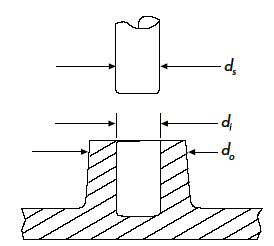
\includegraphics[width=0.5\textwidth]{img/analysis/thruster/pressfit.png}
	\caption{Pressfit Interference Diameters \cite{pressfit}}
	\label{fig:pressfit}
\end{figure}

\begin{equation}
\sigma_a=\frac{d_s-d_i}{d_s}\cdot{}E_p\cdot{}
\frac{d_o^2+d_s^2}{2d_o^2}
\end{equation}

\begin{equation}
i_a=d_s\cdot{}\frac{\sigma_a}{E_p}\cdot{}
\frac{d_o^2+d_s^2}{2d_o^2}
\end{equation}

\begin{equation}
n=\frac{S_y}{\sigma_a}
\end{equation}

Dimensions were taken from the first iteration of the design. Yield stress was estimated as 65MPa for the plastic parts.

\begin{equation*}
\sigma_a=\frac{6mm-(5.8mm)}{6mm}\cdot{}55MPa\cdot{}
\frac{(16mm)^2+(6mm)^2}{2(16mm)^2}=1.04MPa
\end{equation*}

\begin{equation*}
n=\frac{65MPa}{1.04MPa}=62.5
\end{equation*}

\begin{equation*}
i_a=(6mm)\cdot{}\frac{(1.04MPa)}{52.6MPa}\cdot{}
\frac{(16mm)^2+(6mm)^2}{2(16mm)^2}=0.068mm
\end{equation*}
\end{document}